\section{Data Reduction and Analysis} \label{sec:reduction-analysis}
    \begin{itemize}
        \item Will contain the details of the data reduction routines used
        \item Will contain the software tools used for data analysis
    \end{itemize}
    The raw data pertaining to all of the observations were downloaded using the online archival query interface at the \textit{High Energy Astrophysics Science Archive Research Center} (HEASARC)\footnote{\url{https://heasarc.gsfc.nasa.gov/db-perl/W3Browse/w3browse.pl}}. The data was reduced finally to \textit{Flexible Image Transport System} (FITS)\footnote{\url{https://fits.gsfc.nasa.gov/standard40/fits_standard40aa-le.pdf}} format using the software tools for the corresponding observatory with recommended settings in the relevant data analysis threads, wherever available. For the final analysis, a set of four files were generated for each of the observations. As a standard practice, these files were given the extensions as per a convention adopted by the authors as follows:
    \begin{enumerate}
    	\item Source spectrum, with file extension \texttt{.src}
    	\item Background spectrum, with file extension \texttt{.bkg}
    	\item Redistribution matrix file (RMF), with file extension \texttt{.rmf}
    	\item Ancillary response file (ARF), with file extension \texttt{.arf}
    \end{enumerate}
    The above files were grouped using the FTOOLS task \texttt{grphha}\footnote{\url{https://heasarc.gsfc.nasa.gov/docs/heasarc/caldb/docs/memos/cal_sw_93_010/cal_sw_93_010.pdf}} to have an appropriate minimum number of counts per bin. The resulting spectrum sets were analysed using \textit{Xspec} version 12.13.1.
    
    \subsection{XMM-Newton EPIC-pn data reduction}
    	The SSS \source\ was observed by all the instruments, viz. EPIC-MOS 1, EPIC-MOS 2, EPIC-pn and RGS, on-board ESA's XMM-Newton observatory for $\sim 52$ ks on 16 December 2000. Whereas, we had retrieved data from all the instruments, we decided to use only the EPIC-pn data. The reason for this being two-fold:
    	\begin{enumerate}[i.]
    		\item The spectral region of interest is of the lowest energies detectable by EPIC, and the pn detector has a comparatively higher sensitivity than the MOS detectors at lower energies \cite{stecchini2023revisiting,mateos2009statistical}.
    		\item Currently, the high resolution grating spectra (such as those produced by the RGS) yield unacceptable fits to atmosphere models of SSS. Also, no atmosphere model has yet been able to reproduce all the details in such grating spectra \cite{ness2020complications}.
    	\end{enumerate}
    	As per recommendations by the XMM-Newton SOC, the data analysis was restricted to energies above 0.2 keV\footnote{\url{https://xmmweb.esac.esa.int/docs/documents/CAL-TN-0018.pdf}}. The data reduction procedures were performed using the \textit{XMM-Newton Science Analysis System} (SAS) version 21.0.0.
    
    	The Observation Data Files (ODF) were downloaded from HEASARC. In order to prepare the data for processing, we included the instrumental and calibration information by creating a Calibration Index File (CIF), which was up-to-date with the current calibration files (CCF)\footnote{\url{https://www.cosmos.esa.int/web/xmm-newton/current-calibration-files}}, and an extended ODF summary file. These were done by running the SAS tasks \texttt{cifbuild} and \texttt{odfingest} respectively. The ODFs were then reprocessed to generate the calibrated event files using the \texttt{epproc}, using the default parameters. The event file for EPIC-pn was filtered using the canned screening set of flags, and by setting \texttt{PATTERN==0} to select only single-pixel events in order to maximise energy calibration and resolution. The procedure described by Jethwa et al. (2015) \cite{jethwa2015pile} was used to check and find that the spectral distortion and flux loss both $<0.01\%$, which implied that the pile-up effects could be neglected.
	    \begin{figure}[!htb]
	        \centering
	        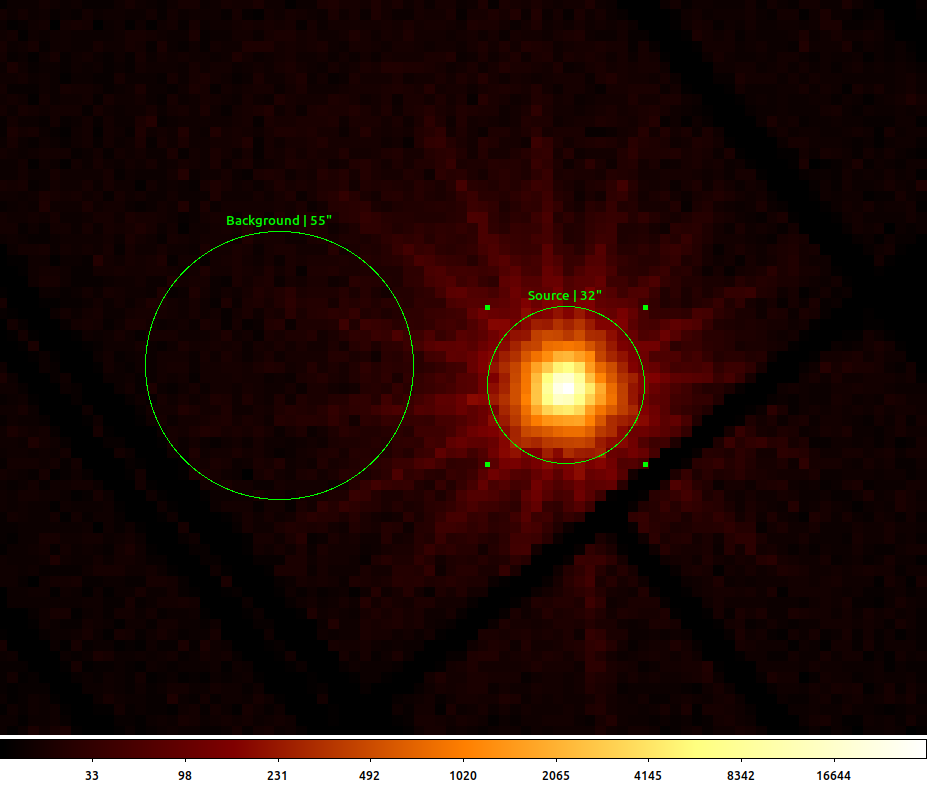
\includegraphics[width=0.45\textwidth]{figures/rx-j0925.7-4758_0111150101_src-bkg.png}
	        \caption{Source and background extraction regions for the XMM-Newton observation of \source}
	        \label{fig:src-bkg:pn}
	    \end{figure}
    
    	The source photons were extracted from a circular region having a radius of 30" which is centred at the \source\ centroid position, encompassing about 85-90\% of XMM-Newton's telescope's on-axis PSF\footnote{\url{https://xmm-tools.cosmos.esa.int/external/xmm_user_support/documentation/uhb/onaxisxraypsf.html}}. For the background photons, first the SAS task \texttt{ebkgreg} was executed to obtain an optimum circular background extraction region of radius $\sim$55". The resulting source and background extraction regions are displayed in figure \ref{fig:src-bkg:pn}. The RMF and ARF were generated using the standard SAS tasks \texttt{rmfgen} and \texttt{arfgen}. The spectrum was finally binned to have a minimum of 10 counts/bin using the task \texttt{grphha} in order to make it ready for analysis using Xspec.
    
    \subsection{ASCA SIS1 data reduction}
    	The SSS \source\ was observed by the SIS1 instrument on-board Japan's ASCA observatory for a total duration of $\sim 21$ ks on 22 December 1994, with the purposes of characterization of its continuum spectral shape and the investigation of absorption edge features \cite{ebisawaAsca2001ApJ}.
    
    \subsection{Chandra ACIS data reduction}
    
    \subsection{NICER XTI data reduction}
    	The SSS \source\ was observed by the XTI instrument on-board the NICER observatory on the International Space Station (ISS) for a total duration of $\sim 21$ ks on three occasions during 18--19 May 2019.
    	
    	The XTI observation dataset and auxiliary files were downloaded from HEASARC. In order to prepare the data for processing, we set up the remote access of the HEASARC CALDB by following the recommended procedure\footnote{\url{https://heasarc.gsfc.nasa.gov/docs/heasarc/caldb/caldb_remote_access.html}}. All data reduction commands for NICER science data are made available with the latest versions of HEASoft\footnote{\url{https://heasarc.gsfc.nasa.gov/docs/software/heasoft/}}. The cleaned event files were extracted using the \texttt{nicerl2} command\footnote{\url{https://heasarc.gsfc.nasa.gov/lheasoft/ftools/headas/nicerl2.html}}. They were then loaded into Xselect\footnote{\url{https://heasarc.gsfc.nasa.gov/ftools/xselect/}}, a multipurpose tool for filtering event files and generating images, spectra, and light curves made available as part of HEASoft. This produces the source and background spectrum files in FITS format. The ARF and RMF were generated with the extracted source spectrum files using the \texttt{nicerarf}\footnote{\url{https://heasarc.gsfc.nasa.gov/lheasoft/ftools/headas/nicerarf.html}} and the \texttt{nicerrmf}\footnote{\url{https://heasarc.gsfc.nasa.gov/lheasoft/ftools/headas/nicerrmf.html}} commands respectively. The spectrum set was finally grouped and binned to a minimum of 10 counts/bin using \texttt{grphha} and made ready for analysis using Xspec.